\documentclass{powerdot}

\pdsetup{lf={Jordan Thayer (Draper)},
	 rf={15 Puzzle}}

% for including postscript
\usepackage{graphicx}
\usepackage{amsmath}
\usepackage{latexsym} %%box def
\usepackage{pstricks,,pst-node,pst-tree}
\usepackage{amssymb}
\DeclareMathOperator*{\argmin}{argmin}
% get my macros

% shorthand for including the figures
\newcommand{\figwidth}[1]{%
	\bc
	\includegraphics[width=\textwidth]{#1}
	\ec
}
\newcommand{\figheight}[1]{%
	\bc
	% height=2.8in
	\includegraphics[height=2.8in]{#1}
	\ec}

\newcommand{\qspace}{\vspace{0.1in}}
\newcommand{\myred}[1]{{\color{red} #1}}
\newcommand{\mygreen}[1]{{\color{green} #1}}
\newcommand{\myyellow}[1]{{\color{yellow} #1}}
\newcommand{\turnred}[1]{{\onslide*{1}{#1}\onslide*{2}{\color{red} #1}}}
\newcommand{\myblue}[1]{{\color{blue} #1}}

\newcommand{\mybf}[1]{\textcolor{red}{\bf #1}}
\newcommand{\myem}[1]{\textcolor{blue}{\em #1}}
\newcommand{\openfH}{{\myit open}_{\widehat{f}}}
\newcommand{\openf}{{\myit open}_f}


\title{AI For Games: What Are We Talking About?}
\author{Jordan Thayer}

\date{\vspace{0.2in}}
\begin{document}
\maketitle

\section[slide=false]{Logistics}
\begin{slide}{Syllabus}
  \begin{enumerate}
    \item Introduction To Games
      \subitem Syllabus
      \subitem Types of Games
      \subitem Terminology
      \subitem Brief History of Games and AI
    \item Minimax Tree Search
    \item $\alpha$-$\beta$ pruning
    \item Multi-Armed Bandits and Monte Carlo Tree Search
    \item Implementing Monte Carlo Tree Search
    \item Weak and Strong Solutions to Games, Checkers
  \end{enumerate}
\end{slide}

\begin{slide}{Today\hfill Introduction to Games}
  \begin{itemize}
    \item Types of Games
    \item Terminology
    \item Brief History of AI and Games
  \end{itemize}
\end{slide}
%%%%%%%%%%%%%%%%%%%%%%%%%%%%%%%%%%%%%%%%%%%%%%%%%%%%%%%%%%%%%%%%%%%
\section{Types of Games}

\begin{slide}{Single Player Games}
  \twocolumn{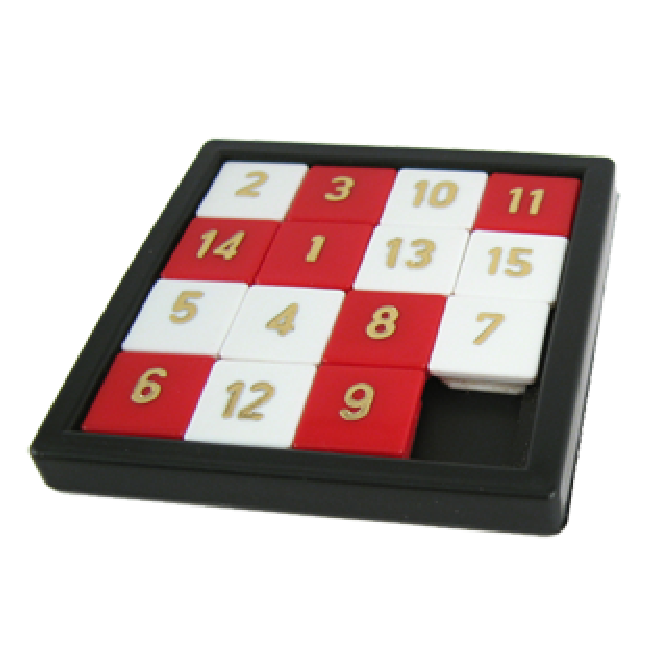
\includegraphics[width=3in]{images/15puz.eps}}
            {
              \begin{itemize}
              \item Foo
              \item Bar
              \end{itemize}
            }
\end{slide}

\begin{slide}{Two Player Games}
  \twocolumn{
    %% Picture of Chess
  }
            {\begin{itemize}
                \item Exactly two players
                \item Usually played in turns
                \item Typically Zero-sum
              \end{itemize}
            }
\end{slide}

\begin{slide}{N-Player Games}
  \twocolumn{
    %% Picture of Catan
  }
            {\begin{itemize}
                \item More Than Two Players
                \item Produces a ranking of players
                \item Coallitions form and disolve during play
              \end{itemize}
            }
\end{slide}

\begin{slide}{Games with Chance}
  \twocolumn{
    %% Picture of Backgammon
  }
  {\begin{itemize}
      \item Dice
      \item Spinners
      \item Shuffling
    \end{itemize}
    }
\end{slide}

\begin{slide}{Games with Imperfect Information}
  \twocolumn{
    %% Picture of Poker
  }
            {\begin{itemize}
                \item Flipping Tiles, Cards
                \item ``Hands''
                \item Asymmetric Information
            \end{itemize}}
\end{slide}

\begin{slide}{Taxonomy of Games and Approaches}
  Games:
  \begin{tabular}{lll}
               & Perfect Information & Imperfect Information \\
    One Player & Permutation Puzzles & Solitaire \\
    Two Player & Chess, Checkers     & Stratego \\
    N Players  & Some Board Games    & Most Card Games \\
  \end{tabular}

  Approaches:
  \begin{tabular}{lll}
               & Perfect Information & Imperfect Information \\
    One Player & Depth First Search & Policy Search \\
    Two Player & Game Tree Search   & MDP \& POMDP Solvers \\
    N Players  & Game Tree Search   & Regret Minimization \\
  \end{tabular}
\end{slide}

%%%%%%%%%%%%%%%%%%%%%%%%%%%%%%%%%%%%%%%%%%%%%%%%%%%%%%%%%%%%%%%%%%%
\section{Two Player Perfect Information Games}

\begin{slide}{Two Player Perfect Information Games}
  \begin{itemize}
    \item Exactly Two Players
    \item All actions are deterministic
    \item Shared game representation
    \item Each game is self contained
  \end{itemize}
\end{slide}

\begin{slide}{Turns and Ply}
  %% Draw an initial game state
  %% Draw player 1s move
  %% Add player twos move
\end{slide}

\begin{slide}{Win, Lose, or Draw}
\end{slide}

\begin{slide}{Tree Search and Graph Search}
  %% Draw the inital game state again
  %% Show each possible first move, setting up a tree of depth 1
  %% Show each possible response, shwoing a tree of depth 2
  %% Show another ply, inducing a DAG
\end{slide}

\begin{slide}{Solutions, Strategies}
  %% Weakly Solved
  %% Strongly Solved
\end{slide}

%%%%%%%%%%%%%%%%%%%%%%%%%%%%%%%%%%%%%%%%%%%%%%%%%%%%%%%%%%%%%%%%%%%
\section{AI and Games}

\begin{slide}{McCarthy Studies Chess Players}
  %% Images of notes taken from players describing how they play
\end{slide}

\begin{slide}{Checkers and the March to Chinook}
  %% Timeline of Sammuelto Schaeffer
\end{slide}

\begin{slide}{More Man Machine Competitions \hfill Deep Blue}
  %% Chess Competition
\end{slide}

\begin{slide}{We're Better at Crosswords}
  %% How we play crosswords, man machine competitions
\end{slide}

\begin{slide}{Bridge Baron}
  %% Nau's planning based approach 
\end{slide}

\begin{slide}{Holdem' Starts to Fall}
\end{slide}

\begin{slide}{Jeopardy!}
\end{slide}

\begin{slide}{Go}
\end{slide}

\begin{slide}{Rock, Paper, Scissiors\hfill Is nothing sacred?}
\end{slide}

\end{document}
